\section{Motivation}
Ganz am Anfang der Einleitung muss in das Thema eingeführt werden. Am besten gehst Du an dieser Stelle davon aus, dass Dein Leser keinerlei Vorkenntnisse mitbringt (auch wenn das selten der Fall sein dürfte). In der Einleitung einer Seminararbeit wird außerdem genau beschrieben, welche Fragestellung beantwortet werden soll. Begründe Deine Eingrenzung des Themas und erläutere, wie Du beim Sammeln der Literatur und gegebenenfalls beim Erheben von Daten oder Analysen vorgegangen bist.
\begin{itemize}
	\item Normale Software wird so gebaut und evaluiert, sodass sie funktioniert
	\item “If you start with an English-language specification, you’re inherently starting with an ambiguous specification,” said Jeannette Wing, corporate vice president at Microsoft Research. “Any natural language is inherently ambiguous. In a formal specification you’re writing down a precise specification based on mathematics to explain what it is you want the program to do.”
	\item \url{https://www.quantamagazine.org/formal-verification-creates-hacker-proof-code-20160920/}
	\item Fehler 40
	\item Was wenn ein Compiler auf unterschiedlichen System aus dem selben Sourcecode unterschiedliche Runnables macht?
	\item \url{https://www.mikrocontroller.net/articles/Compilerfehler}
	\item \url{https://blog.regehr.org/archives/26}
	\item Unit tests schreiben, um möglichst viele Fehler zu finden -> Proof Assistent um für alle korrekt zu funktionieren
	\item Proof Assistent benutzen um formal richtigen Code zu schreiben/generieren
	\item \textbf{Fragestellung: Wie gewährleiste ich sichereren/gut getesteten Code?}
\end{itemize}


\section{Grundlagen}
\subsection{Was ist ein Proof Assisstant}
\url{https://www.youtube.com/watch?v=95VlaZTaWgc&t=2646s}
\subsubsection{Proof Verifier}
\subsubsection{Theorem Provers}

\subsection{Übersicht}
\url{https://en.wikipedia.org/wiki/Proof_assistant}
\begin{itemize}
	\item ACL2
	\item Isabelle
	\item Coq
\end{itemize}

\section{Coq}
\url{https://www.amazon.de/Certified-Programming-Dependent-Types-Introduction/dp/0262026651/ref=sr_1_fkmr0_1?__mk_de_DE=ÅMÅŽÕÑ&keywords=coq+proof+assistent&qid=1572974699&sr=8-1-fkmr0}
\begin{itemize}
	\item Warum Coq
	\item funktionaler Programmierstil
	\item Dependent type Sprache
	\item Frenchmade
	\item Warum ist coq so erfolgreich?
\end{itemize}

\section{Programmatische Coq-Grundlagen}
\subsection{funktionaler Programmierstil}
\subsection{Basisbegriffe}
\url{https://softwarefoundations.cis.upenn.edu/lf-current/Basics.html#lab18}
\begin{itemize}
	\item Funktion
	\item Taktik
	\item Ziel
	\item Subgoal
	\item Proof/Beweis
\end{itemize}
\subsection{Sprache}
\subsection{Beispielbeweise}

\begin{lstlisting}[language=coq,firstnumber=1,caption=Coq Beispiel,label=lst:api-config]
	Inductive day : Type :=
	| monday
	| tuesday
	| wednesday
	| thursday
	| friday
	| saturday
	| sunday.

	Definition next_weekday (d:day) : day :=
	match d with
	| monday => tuesday
	| tuesday => wednesday
	| wednesday => thursday
	| thursday => friday
	| friday => monday
	| saturday => monday
	| sunday => monday
	end.

	Compute (next_weekday friday).
	(* ==> monday : day *)
	Compute (next_weekday (next_weekday saturday)).
	(* ==> tuesday : day *)
\end{lstlisting}

\section{Zusammenspiel Proof - Program}
\begin{itemize}
	\item Wir haben eine Liste von Dingen, die die Software tun soll, und verwenden Logik, um zu beweisen, dass die Software diese Dinge tut.
	\item \url{https://www.youtube.com/watch?v=Ue8QG8pf0wU}
	\item Codegenerierung, Proof -> Program
	\item Programm -> Proof
	\item Beispiel mit Liste aus Video
\end{itemize}

\subsection{How-to}
\begin{itemize}
	\item \url{https://medium.com/@ahelwer/formal-verification-casually-explained-3fb4fef2e69a}
	\item Erstelle eine Spezifikation, die ein Programm beschreibt
	\item Schreie die Spezifikation mathematisch in ein Proof Tool
	\item Wenn es Fehler enthält, sagt es dir der Verifier
	\item 
\end{itemize}

\section{Aktuelle Anwendung}
\subsection{Proofed Stack}
\begin{itemize}
	\item CompCert (C compiler)
	\item Princeton VST
	\item Certikos (verified Operating System with hypervisor and multi instances)
	\item \url{http://plv.csail.mit.edu/kami/}
	\item \url{https://www.zdnet.com/article/certikos-a-hacker-proof-os/}
	\item \url{https://github.com/PrincetonUniversity/VST}
	\item \url{https://vst.cs.princeton.edu}
	\item \url{https://news.yale.edu/2016/11/14/certikos-breakthrough-toward-hacker-resistant-operating-systems}
\end{itemize}
\subsection{CompCert for C}
\url{http://compcert.inria.fr}
\subsection{JSCert for ECMA 5}
\url{https://github.com/jscert/jscert}
\subsection{4-Farben Rätsel ist löstbar!}
\subsection{CertiCoq}
\url{https://www.cs.princeton.edu/~appel/papers/certicoq-coqpl.pdf}

\section{Anwendbarkeit in der Praxis}
\begin{itemize}
	\item Objektorientierung
	\item Sicherheitskritische Systeme
	\item Compilerbau
\end{itemize}


\section{Fazit}
\subsection{Aussicht}

\section{Glossar}


\section{Einleitung}
\label{s:intro}

Hier kommt die Einleitung.


%%%%%%%%%%%%%%%%%%%%%%%%%%%%%%%%%%%%%%%%%%%%%%%%%%%%%%%%%%%%%%
\subsection{Ein Abschnitt der Einleitung}
\label{ss:intro:abc}

Einen Überblick findet man z.\,B.\ in \cite{Auer00:HTF}.

\begin{figure}[t]
	\centering
	
	\begin{subfigure}{0.45\linewidth}
		\centering
		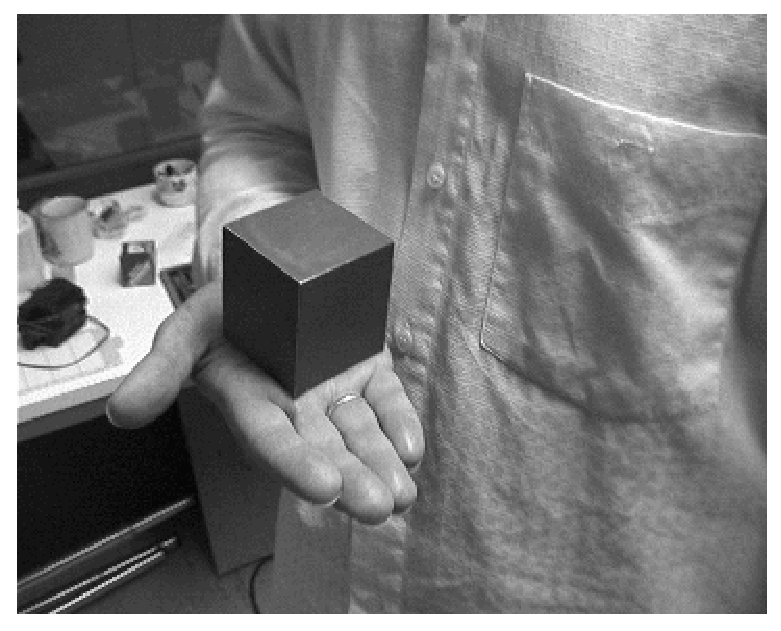
\includegraphics[width=\linewidth]{\figdir/handorig}
		\caption{Originalbild}
		\label{FIG:arexorig}
	\end{subfigure}
	%
	\begin{subfigure}{0.45\linewidth}
		\centering
		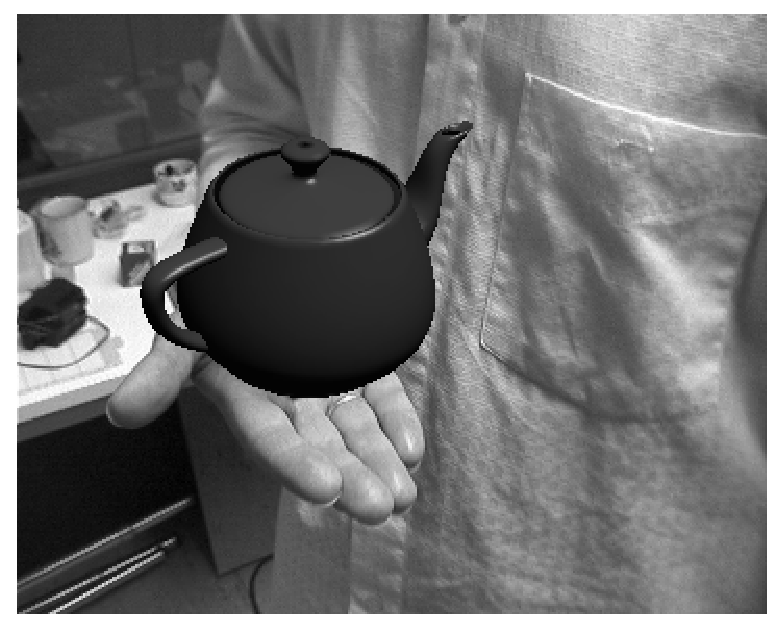
\includegraphics[width=\linewidth]{\figdir/handaug}
		\caption{erweitertes Bild}
		\label{FIG:arexaugm}
	\end{subfigure}
	%
	\caption[AR Beispiel]
	{Beispiel eines Augmented Reality Systems: es folgt eine Beschreibung (Bilder aus \cite{Schmidt01:PAO})}
	\label{FIG:arex}
\end{figure}

Ein Beispiel wird in Abb.\ \ref{FIG:arex} gezeigt.
Das verwendete Objekt ist in Abb.\ \ref{FIG:arexorig} dargestellt, das Ergebnis in Abb.\ \ref{FIG:arexaugm}.

Eine Formel
\begin{equation}
\label{eq:cvp:test}
f(x) = \frac{1}{3} x + 5, \quad x \in \real.
\end{equation}

Und noch eine:
\begin{equation}
\label{eq:cvp:matvec}
\bm{M}  = \bm{Ax} \pi, \quad \bm{A} \in \real^{2 \times 2}, \bm{x} \in \real^2.
\end{equation}

Tabelle \ref{t:CodebookOverview} gibt einen Überblick über XYZ.

\begin{table}[t]
	\centering\small
	%
% generated by TexTableGenerator.pl ((c) Florian Vogt)
% from file: /home/Jochen/data/dissdata/results/CodebookOverview.log
%
\begin{tabular}{l|ccc|cc}
\hline
\hline
                  \textbf{Sequence} &          ARTS &           wman &         stcams &         ARTVZ &        ARTSUZ \\ 
                 \textbf{\# Frames} &             190 &              40 &             400 &             270 &             190 \\ 
     \textbf{\# relative movements} &           17955 &             780 &           79800 &           36315 &           17955 \\ 
\textbf{\# movements after pre-sel.} &           14336 &             623 &           37915 &           21788 &           14343 \\ 
       \textbf{min.\ angle in seq.} &   0.233$^\circ$ &    5.95$^\circ$ &   0.154$^\circ$ & 0.00000171$^\circ$ &  0.0388$^\circ$ \\ 
       \textbf{max.\ angle in seq.} &    81.7$^\circ$ &     180$^\circ$ &    47.3$^\circ$ &    80.3$^\circ$ &    80.9$^\circ$ \\ 
\textbf{min.\ angle after pre-sel.} &    12.9$^\circ$ &    21.1$^\circ$ &    17.3$^\circ$ &    16.3$^\circ$ &    12.9$^\circ$ \\ 
\textbf{max.\ angle after pre-sel.} &    81.7$^\circ$ &     161$^\circ$ &    47.3$^\circ$ &    80.3$^\circ$ &    80.9$^\circ$ \\ \hline\hline
\end{tabular}

	\caption[Testtabelle]{Datenselektion für verschiedene Testdatensätze.}
	\label{t:CodebookOverview}
\end{table}


%%% Local Variables: 
%%% mode: latex
%%% TeX-master: "thesis.tex"
%%% End: 
